\chapter{Analyzing Electrical Networks - Basic Principles}
In this chapter, we'll use three fundamental principles to analyze electrical networks (circuits). Some of these tools apply to other types of networks as well.

\par
\section{Basic Principles}
These principles lead to constraints (limitations) as to what voltage or current values the electrical network can have. Constraints lead to equations. Constraints help us narrow in on how the circuit must behave.

\begin{enumerate}
\item Net Current into a node equals zero. ($\sum{I_{IN}}=0$) \underline{Be careful, not always true.}
\item Voltage around loop equals zero. ($\sum{V_{LOOP}}=0$) \underline{Be careful, not always true.}
\item Power In = Power Out (Conservation of Energy). \underline{Be careful!}
\end{enumerate}

%%%%%%%%%%%%%%%%%%%%%%%%%%%%%%%%%%%%%%%%%%%%%
\subsection{Basic Tool I. Net current in equals zero.}
According to this principle, the currents into a node must equal the currents leaving that node. This assumes two things:

\begin{itemize}
\item That the charge at the node can not increase or decrease significantly. It certainly can't increase forever\footnote{If infinite charge were to accumulate on a node, it would take infinite energy to add more charge to it - good luck with that.}. For our traffic network, this principle would apply if none of the towns had any parking. In that case, the cars entering the town must always match the number of cars leaving the town.
\item That charge can not be created or destroyed - or that electric charge is conserved. Were it not for this, charge could go into a node and be destroyed, like gargabe going into an incinerator.
\end{itemize}
\par

\begin{bigidea}
Look to identify conserved quantities, like electric charge. Conserved quantities lead to constraints and equations that describe the system.
\end{bigidea}

\par
If you consider items leaving as equivalent to a negative number of items entering, then the in=out principle this can be restated as the sum of all items entering must be zero. This relationship is sometimes called Kirchoff's Current Law, or KCL.
\par
\begin{align*}
\Sigma I_{entering}=0	&&\text{KCL}
\end{align*}

KCL holds for each node, so if a circuit has 5 nodes, you get 5 equations.

\begin{blevel}
A box begins with 20C of charge. 5 Amps enters the box for 2 minutes, then 10 minutes later 7 Amps leaves the box for 1 minute. Determine the final amount of charge in the box.
\end{blevel}

\begin{dlevel}
Conservation of mass can be useful. Does it always apply? If not, when would it not apply? Would it apply when tracking all the food entering and leaving a cafeteria? If not, what would you need to do to make it apply?
\end{dlevel}

\begin{blevel}
Determine which these situations would be consistent or approximately consistent with the in=out principle:
\begin{itemize}
\item Total gasoline going into and out of a car.
\item Electric charge going into and out of a node.
\item Gasoline going into and out of a gas station.
\item The mass of water going into and out of a plumbing junction.
\end{itemize}
\end{blevel}

%%%%%%%%%%%%%%%%%%%%%%%%%%%%%%%%%%%%%%%
\subsection{Basic Tool II. Voltage around loop equals zero.}
In our hiking trail example earlier, if you start hiking at point A and end at point A, the total change in elevation would be zero. Therefore the total change in gravitational potential (gravitational potential energy per mass) would be zero. We can generalize this statement for trail networks as follows:
\par

\begin{align}
\Sigma V_g(loop)=0	&&\text{Trail System Law}
\end{align}

A similar rule holds for electrical networks, and for the same reasons. This is sometimes called Kirchoff's Voltage Law. 

\begin{align}
\Sigma V(loop)=0	&&\text{KVL}
\end{align}

Unfortunately, like KCL, KVL is also not always true\footnote{Whether or not it is unfortunate depends on your point of view. The exceptions to this rule are pretty important to how the whole world works.}. The presence of changing magnetic fields can cause the sum of the voltages around a loop to be other than zero.

\subsection{Basic Tool III. Power In = Power Out (Conservation of Energy)}
For closed systems, the total energy of the system must be fixed (principle of conservation of energy). If there is energy entering the system, like via a current or voltage source, then that energy must be going somewhere \footnote{I don't like this verbage "going somewhere" - I think I'd prefer to say something like transformed somewhere. I'm sure there's a better way to say this without giving a misleading impression that little particles of energy are moving around the circuit, like the flow of charge.}, like being absorbed by a resistor or stretching a spring.

\section{Sample Circuit}
We will now analyze the circuit in Figure~\ref{F:3CKT} using the above tools. We'll introduce a make-believe component called a \emph{Gator}, indicated by the $\Rightarrow$ symbol. A Gator behaves such that there is always a 2V drop across it (the arrow points to the more positive side).

\par
The voltage V is +5V.
\par

\begin{figure}[H]
\begin{center}
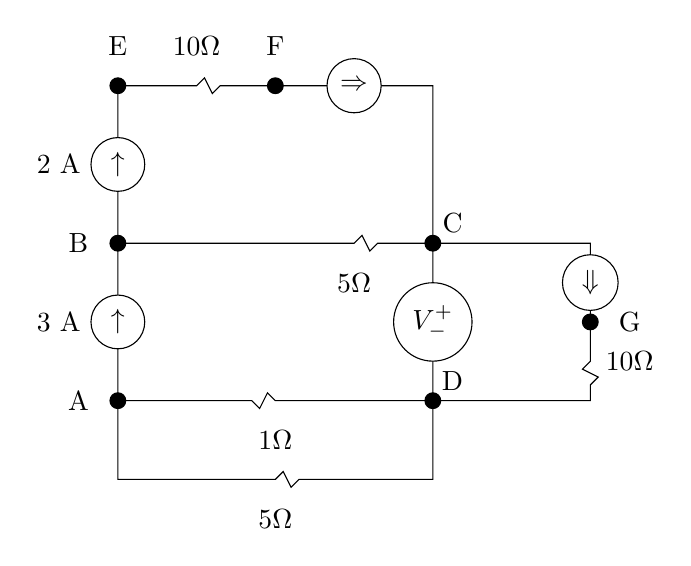
\begin{tikzpicture}
\draw (1,0)--(1,1) node[circle, draw=black, radius=2cm, fill=white]{$\uparrow$}
--(1,2)--(4,2)--(4.1,2.1)--(4.2,1.9)--(4.3,2)--(5,2);
\node at (4,1.5) {$5 \Omega$};
\node at (0.25,1) {3 A};
\node at (0.25,3) {2 A};
\node at (7.5,.5) {$10 \Omega$};
\node at (2,4.5) {$10 \Omega$};
\node at (3,-.5) {$1 \Omega$};
\node at (3,-1.5) {$5 \Omega$};
\filldraw (1,0) circle[radius=1 mm];
\node at (.5,0) {A};
\filldraw (1,2) circle[radius=1 mm];
\node at (.5,2) {B};
\filldraw (5,2) circle[radius=1 mm];
\node at (5.25,2.25) {C};
\filldraw (5,0) circle[radius=1 mm];
\node at (5.25,.25) {D};
\filldraw (1,4) circle[radius=1 mm];
\node at (1,4.5) {E};
\filldraw (3,4) circle[radius=1 mm];
\node at (3,4.5) {F};
\filldraw (7,1) circle[radius=1 mm];
\node at (7.5,1) {G};
\draw (1,2)--(1,3) node[circle, draw=black, radius=2cm, fill=white]{$\uparrow$}
--(1,4)--(2,4)--(2.1,4.1)--(2.2,3.9)--(2.3,4)
--(4,4) node[circle, draw=black,radius=2cm, fill=white]{$\Rightarrow$}
--(5,4)--(5,2)
--(5,1) node[circle, draw=black, radius=2cm, fill=white]{$V_{-}^{+}$}
--(5,0)--(3,0)--(2.9,.1)--(2.8,-.1)--(2.7,0)--(1,0);
\draw (5,2)--(7,2)
--(7,1.5) node[circle, draw=black,radius=2cm, fill=white]{$\Downarrow$}
--(7,.5)--(6.9,.4)--(7.1,.3)--(7,.2)--(7,0)--(5,0);
\draw (1,0)--(1,-1)--(3,-1)--(3.1,-.9)--(3.2,-1.1)--(3.3,-1)--(5,-1)--(5,0);
\end{tikzpicture}
\caption{A circuit for analysis.}
\label{F:3CKT}
\end{center}
\end{figure}

There are many places to start, so the plan outlined in this example is just one way to do it.

\begin{enumerate}
\item Find the current from B to C. Use KCL.
\item Use Ohm's Law to determine the voltage drop from B to C. For a resistor, a positive current will always flow from a positive voltage to negative voltage.\footnote{For sources, the current can flow either direction depending on whether the source is absorbing power or producing power.}
\item Identify the current from E to F. Use Ohm's Law to determine the voltage $V_{EF}$.
\item Use KVL to determine the voltage drop across the 2A current source.
\item Use KVL to determine the voltage drop across the 10 Ohm resistor, $V_{GD}$.
\item Use Ohm's Law to determine the current from node G to node D (through the 10 Ohm resistor).
\end{enumerate}

Answers are now in blue.

\begin{figure}[H]
\begin{center}
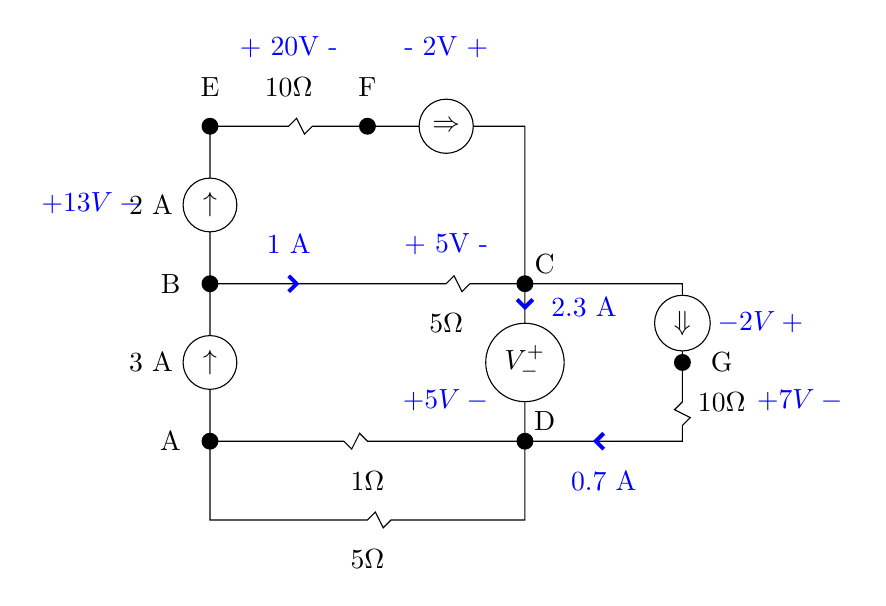
\begin{tikzpicture}
\draw (1,0)--(1,1) node[circle, draw=black, radius=2cm, fill=white]{$\uparrow$}
--(1,2)--(4,2)--(4.1,2.1)--(4.2,1.9)--(4.3,2)--(5,2);
\node at (4,1.5) {$5 \Omega$};
\node at (0.25,1) {3 A};
\node at (0.25,3) {2 A};
\node at (7.5,.5) {$10 \Omega$};
\node at (2,4.5) {$10 \Omega$};
\node at (3,-.5) {$1 \Omega$};
\node at (3,-1.5) {$5 \Omega$};
\filldraw (1,0) circle[radius=1 mm];
\node at (.5,0) {A};
\filldraw (1,2) circle[radius=1 mm];
\node at (.5,2) {B};
\filldraw (5,2) circle[radius=1 mm];
\node at (5.25,2.25) {C};
\filldraw (5,0) circle[radius=1 mm];
\node at (5.25,.25) {D};
\filldraw (1,4) circle[radius=1 mm];
\node at (1,4.5) {E};
\filldraw (3,4) circle[radius=1 mm];
\node at (3,4.5) {F};
\filldraw (7,1) circle[radius=1 mm];
\node at (7.5,1) {G};
\draw (1,2)--(1,3) node[circle, draw=black, radius=2cm, fill=white]{$\uparrow$}
--(1,4)--(2,4)--(2.1,4.1)--(2.2,3.9)--(2.3,4)
--(4,4) node[circle, draw=black,radius=2cm, fill=white]{$\Rightarrow$}
--(5,4)--(5,2)
--(5,1) node[circle, draw=black, radius=2cm, fill=white]{$V_{-}^{+}$}
--(5,0)--(3,0)--(2.9,.1)--(2.8,-.1)--(2.7,0)--(1,0);
\draw (5,2)--(7,2)
--(7,1.5) node[circle, draw=black,radius=2cm, fill=white]{$\Downarrow$}
--(7,.5)--(6.9,.4)--(7.1,.3)--(7,.2)--(7,0)--(5,0);
\draw (1,0)--(1,-1)--(3,-1)--(3.1,-.9)--(3.2,-1.1)--(3.3,-1)--(5,-1)--(5,0);
\draw [draw=blue, line width=0.5mm] (2,2.1)--(2.1,2)--(2,1.9);
\node [text=blue] at (2,2.5) {1 A};
\draw [draw=blue, line width=0.5mm] (6,.1)--(5.9,0)--(6,-.1);
\node [text=blue] at (6,-.5) {0.7 A};
\draw [draw=blue, line width=0.5mm] (4.9,1.8)--(5,1.7)--(5.1,1.8);
\node [text=blue] at (5.75,1.7) {2.3 A};
\node [text=blue] at (2,5) {+ 20V -};
\node [text=blue] at (4,5) {- 2V +};
\node [text=blue] at (4,2.5) {+ 5V -};
\node [text=blue] at (-.5,3) {$\begin{matrix}+\\13V\\-\\\end{matrix}$};
\node [text=blue] at (8,1.5) {$\begin{matrix}-\\2V\\+\\\end{matrix}$};
\node [text=blue] at (4,.5) {$\begin{matrix}+\\5V\\-\\\end{matrix}$};
\node [text=blue] at (8.5,.5) {$\begin{matrix}+\\7V\\-\\\end{matrix}$};
\end{tikzpicture}
\caption{The circuit with most of the solutions.}
\label{F:3CKTb}
\end{center}
\end{figure}

We've got \emph{almost} everything, but we're still missing the voltages across and currents through the 1 $\Omega$ and 5 $\Omega$ resistors. It seems like we can't get those values in one easy step, like we did for the others. But don't worry, we just need to write down what we know and then do a little algebra.
\par

Here's what we know.
\begin{itemize}
\item From KCL, the currents $I_1$ (the current through the 1$\Omega$ resistor) and $I_5$ (the current through the 5$\Omega$ resistor) must add up to 3A. $I_1+I_5=3$
\item From Ohm's Law, we know that $V_{AD}=I_1*1$ and $V_{AD}=I_5*5$. 
\item We have three equations and three uknowns. We can solve. 
\end{itemize} 

\begin{blevel}
Solve for $I_1,I_5,V_{AD}$. 
\end{blevel}

\begin{clevel}
Use this answer and KVL to determine the voltage across the 3A current source.
\end{clevel}

Finally, we check our answer using conservation of energy/power (basic tool III). 
\begin{clevel}
Fill in Table~\ref{F:3CKT3}.
\end{clevel}

\begin{table}[H]
\begin{center}
\begin{tabular}{|c|c|c|c|} \hline
component &	current through it	& voltage across it	& power consumed \\ \hline
2A source	&+2A			&-13V (V, I in opp. dirs.)	&-26Watts\\ \hline
3A source	&			&	&	\\ \hline
10 Ohm (E-F)	&+2A			&+20V	&+40W	\\ \hline
5 Ohm (B-C)	&			&	&	\\ \hline
10 Ohm (G-D)	&			&	&	\\ \hline
1 Ohm (A-D)	&			&	&	\\ \hline
5 Ohm (A-D)	&			&	&	\\ \hline
5V source	&			&	&	\\ \hline
Gator Top	&			&	&	\\ \hline
Gator Side	&			&	&	\\ \hline
\end{tabular}
\caption{Table to check conservation of energy.}
\label{F:3CKT3}
\end{center}
\end{table}

\begin{clevel}
What does your total power sum to? It should be zero if the power produced matches the power consumed.
\end{clevel}

\begin{clevel}
Recreate a duplicate of the Table~\ref{F:3CKT3} but for the case where every resistor has a value of 10 Ohms.
\end{clevel}

%%%%%%%%%%%%%%%%%%%%%%%%%%%%%%%%%%%%%%%%%%%%%%%%%%%%%%%%%%%%
\section{Equivalent Combinations}
In this section, we'll look for ways to save time by simplifying a circuit. We'll simplfy by finding a simpler circuit that is equivalent. This is exactly what you do in algebra when you simplify $3x+4x$ by writing $7x$. The $7x$ is often simpler to work with and is mathematically equivalent.

\begin{bigidea}
Look for ways to simplify a problem.
\end{bigidea}

We'll combine resistors that are in series and resistors in parallel. Let's start with a series combination. 
\par

%%%%%%%%%%%%%%%%%%%%%%%%%%%%%%%%%%%%%%%%%%%%%%%%%
\subsection{Series combination}
Two two-terminal components are in series if:
\begin{itemize}
\item One side of one component shares a node with one side of the other component.
\item No other wires are connected to the shared node \footnote{There just can't be any other current leaving the shared node. A wire carrying no current could connect to the shared node.}.
\end{itemize}

We'd like to replace the series combination of two resistors, $R_1$ and $R_2$ with one resistor in such a way as make the two circuits equivalent. The two circuits shown in Figure~\ref{F:2SER} must have the same voltages from A to C and the same current from A to C.

\begin{figure}[H]
\begin{center}
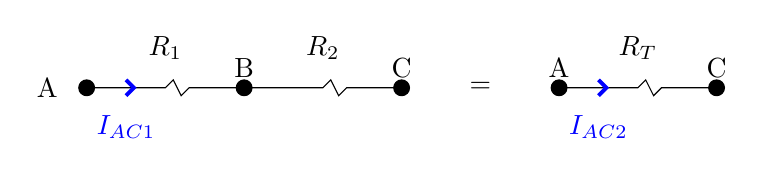
\begin{tikzpicture}
\node at (2,.5) {$R_1$};
\node at (4,.5) {$R_2$};
\filldraw (1,0) circle[radius=1 mm];
\node at (.5,0) {A};
\filldraw (3,0) circle[radius=1 mm];
\node at (3,.25) {B};
\filldraw (5,0) circle[radius=1 mm];
\node at (5,.25) {C};
\draw (1,0)--(2,0)--(2.1,.1)--(2.2,-.1)--(2.3,0)--(3,0);
\draw (3,0)--(4,0)--(4.1,.1)--(4.2,-.1)--(4.3,0)--(5,0);
\draw [draw=blue, line width=0.5mm] (1.5,.1)--(1.6,0)--(1.5,-.1);
\node [text=blue] at (1.5,-.5) {$I_{AC1}$};
\node at (6,0) {=};
%
\node at (8,.5) {$R_T$};
\filldraw (7,0) circle[radius=1 mm];
\node at (7,0.25) {A};
\filldraw (9,0) circle[radius=1 mm];
\node at (9,.25) {C};
\draw (7,0)--(8,0)--(8.1,.1)--(8.2,-.1)--(8.3,0)--(9,0);
\draw [draw=blue, line width=0.5mm] (7.5,.1)--(7.6,0)--(7.5,-.1);
\node [text=blue] at (7.5,-.5) {$I_{AC2}$};
\end{tikzpicture}
\caption{A series combination of resistors and its equivalent resistance.}
\label{F:2SER}
\end{center}
\end{figure}

To determine the combined resistance, $R_T$, we'll do the following:
\begin{enumerate}
\item Observe that to be equivalent: $I_{AC1}=I_{AC2}=I_{AC}$.
\item Observate that to be equivalent $V_{AC}$ must be the same for both.
\item By Ohm's Law, $V_{AC2}=I_{AC}*R_T$
\item By Ohm's Law and KVL\footnote{By KVL, $V_{AC}$ must match $V_{AB}+V_{BC}$}, $V_{AC}=I_{AC}*R_1+I_{AC}*R_2$.
\item Therefore, $I_{AC}*R_T=I_{AC}*R_1+I_{AC}*R_2$.
\item Factor out $I_{AC}$ and cancel. 
\item Conclusion: $R_T=R_1+R_2$.
\end{enumerate}

\begin{clevel}
Prove that for three resistors in series: $R_T=R_1+R_2+R_3$
\end{clevel}

%%%%%%%%%%%%%%%%%%%%%%%%%%%%%%%%%%%%%%%%%%%%%%%%%%%%%%%%
\subsection{Parallel Combination}
Two two-terminal components are in parallel if:
\begin{itemize}
\item One side of one component shares a node with one side of the other component (they are touching).
\item The other two terminals of the two components also share a node (are touching).
\end{itemize}

\begin{clevel}
Use a similar strategy to prove the for two resistors in parallel, $\frac{1}{R_T}=\frac{1}{R_1}+\frac{1}{R_2}$.
\end{clevel}

\begin{clevel}
Starting with: $\frac{1}{R_T}=\frac{1}{R_1}+\frac{1}{R_2}$, use algebra to show that $R_T=\frac{R_1 R_2}{R_1+R_2}$.
\end{clevel}

\begin{blevel}
Make a units based arguement that for three resistors in parallel, the following equation can't possibly be correct (no matter how much you want it to be.) $R_T=\frac{R_1 R_2 R_3}{R_1+R_2+R_3}$.
\end{blevel}

\begin{blevel}
Suppose you start with one resistor and then add another resistor in parallel to it. Does this make the combined resistance, go up, go down, or sometimes go up or down depending on the sizes of the two resistors?
\end{blevel}

\begin{dlevel}
Symmetric polynomials are polynomials where the variables can be swapped without changing the result. For example, $xy+xz+yz$ is a symmetry polynomial, but $xy+x$ is not. Consider four resistors in parallel. Define the symmetry polynomials:
\begin{align}
S_1&=R_1+R_2+R_3+R_4 \\
S_2&=R_1R_2+R_1R_3+R_1R_4+R_2R_3+R_2R_4+R_3R_4\\
S_3&=R_1R_2R_3+R_1R_2R_4+R_1R_3R_4+R_2R_3R_4\\
S_4&=R_1R_2R_3R_4
\end{align}
Show that the equivalent parallel combination is:$R_T = \frac{S_4}{S_3}$. In terms of the symmetry polynomials, what will be the parallel combination of N resistors in parallel?
\end{dlevel}

Consider the following diagram:

\begin{figure}[H]
\begin{center}
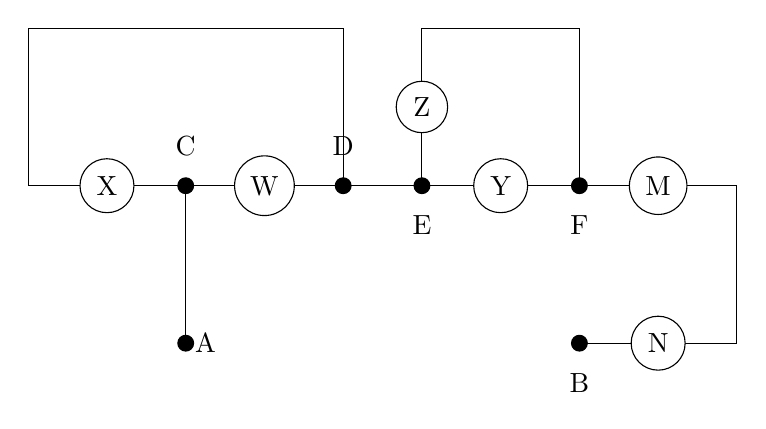
\begin{tikzpicture}
\draw (0,-2)--(0,0)--(-1,0) node[circle, draw=black,radius=2cm, fill=white]{X}
--(-2,0)--(-2,2)--(2,2)--(2,0)--(3,0)
--(4,0)node[circle, draw=black,radius=2cm, fill=white]{Y}
--(5,0)--(6,0)node[circle, draw=black,radius=2cm, fill=white]{M}
--(7,0)--(7,-2)--(6,-2)node[circle, draw=black,radius=2cm, fill=white]{N} 
--(5,-2);
\draw (0,0)--(1,0)node[circle, draw=black,radius=2cm, fill=white]{W}
--(2,0); 
\draw (3,0)--(3,1)node[circle, draw=black,radius=2cm, fill=white]{Z}
--(3,2)--(5,2)--(5,0);
\filldraw (0,-2) circle[radius=1 mm];
\node at (0.25,-2) {A};
\filldraw (5,-2) circle[radius=1 mm];
\node at (5,-2.5) {B};
\filldraw (0,0) circle[radius=1 mm];
\node at (0,.5) {C};
\filldraw (2,0) circle[radius=1 mm];
\node at (2,.5) {D};
\filldraw (3,0) circle[radius=1 mm];
\node at (3,-.5) {E};
\filldraw (5,0) circle[radius=1 mm];
\node at (5,-.5) {F};
\end{tikzpicture}
\caption{Series and Parallel Combination of Components.}
\end{center}
\end{figure}

\begin{clevel}
Fill in the Table~\ref{T:3SP} by identifying which components are in series, parallel or neither.
\end{clevel}

\begin{table}[H]
\begin{center}
\begin{tabular}{|c|c|} \hline
components & series, parallel or neither \\ \hline
X and W &	\\ \hline
Z and W &	\\ \hline
Y and M &	\\ \hline
N and M &	\\ \hline
Z and Y &	\\ \hline
X and M &	\\ \hline
\end{tabular}
\caption{Series or parallel?}
\label{T:3SP}
\end{center}
\end{table}

\begin{clevel}
Suppose components X,Y,W,Z,M and N were are resistors of value 10 Ohms. Determine the value of their combined resistance as measured from node A to B.
\end{clevel}

\begin{blevel}
Draw a way to connect three 5 $\Omega$ resistors to create exactly 7.5 $\Omega$ of total resistance.
\end{blevel}

\begin{alevel}
Suppose current had to flow through a resistor from A to B. If additional resistors were added in series, would this make it easier or harder for current to flow?
\end{alevel}

\begin{clevel}
Consider the infinite resistor network shown in Figure~\ref{F:3TRANS}. All resistors are of size R. Determine the resistance from A to B, called $R_{AB}$. Hint: Because the network is infinite, the resistance to the right of C and D, $R_{CD}$, must equal $R_{AB}$. Write down $R_{AB}$ in terms of itself and solve. If you end with a quadratic equation, you're on the right track.
\end{clevel}

\begin{figure}[H]
\begin{center}
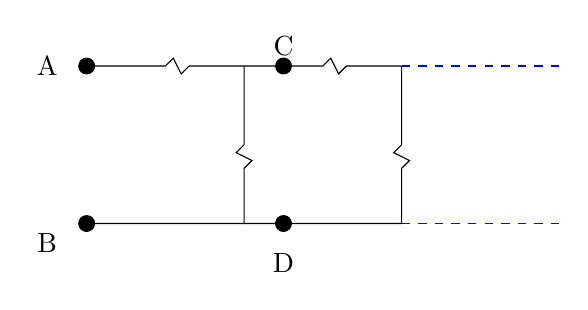
\begin{tikzpicture}
\filldraw (0,0) circle[radius=1 mm]; \draw node at (-.5,-.25) {B};
\filldraw (0,2) circle[radius=1 mm]; \draw node at (-.5,2) {A};
\filldraw (2.5,2) circle[radius=1 mm]; \draw node at (2.5,2.25) {C};
\filldraw (2.5,0) circle[radius=1 mm]; \draw node at (2.5,-.5) {D};
\draw (0,2)--(1,2)--(1.1,2.1)--(1.2,1.9)--(1.3,2)--(2,2);
\draw (2,2)--(2,1)--(1.9,.9)--(2.1,.8)--(2,.7)--(2,0)--(0,0);
\draw (2,2)--(3,2)--(3.1,2.1)--(3.2,1.9)--(3.3,2)--(4,2);
\draw (4,2)--(4,1)--(3.9,.9)--(4.1,.8)--(4,.7)--(4,0)--(2,0);
\draw [dashed, draw=blue] (4,2)--(6,2) (4,0)--(6,0);
\end{tikzpicture}
\caption{Infinite resistive transmission line network.}
\label{F:3TRANS}
\end{center}
\end{figure}

%%%%%%%%%%%%%%%%%%%%%%%%%%%%%%%%%%%%%%%%%%%%%%%%%%%%%%%%%
\subsection{Trust Networks}
Let's apply what we've learned about combining resistors to another type of network, a trust network. Trust networks can involve series and parallel combinations of trust. For example, if A tells B something and B tells C, this means that C must trust both A and B in order to trust the information. This situation represents a series chain of trust.\par

On the other hand, suppose A tells C and also B tells C, and A and B are independent sources \footnote{The idea of independence is important in algebra. In algebra it means that equations are not copies or combinations of each other. In this context, it means basically the same thing, that A and B each have their own reasons for believing something. It's not just that A told B and then they both told you.} then this would represent a parallel chain of trust.\\
\\
We can create a trust diagram, like a circuit diagram. Nodes represent people, or sources of information (like a newspaper). Informations flows on the edges. The edge components represent resistance to the flow of information, or distrust. We'll call them \emph{distrusters} instead of resistors. Series combinations make trust more difficult (distrust adds in series). Parallel combinations make the flow of information easier (more trust, less distrust) because there are more sources conveying the same thing. Figure~\ref{F:3T} shows an example.

\begin{figure}[H]
\begin{center}
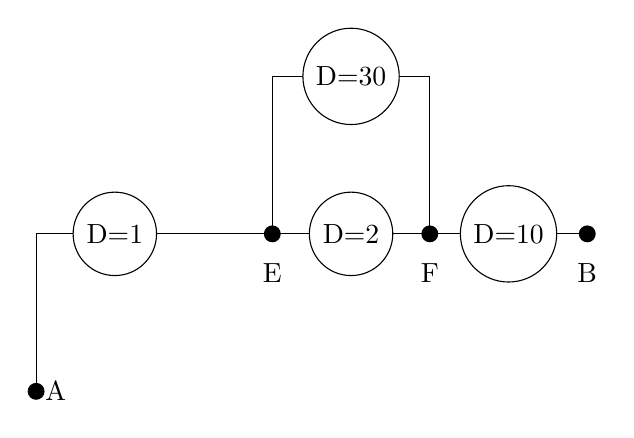
\begin{tikzpicture}
\filldraw (0,-2) circle[radius=1 mm];
\node at (0.25,-2) {A};
\draw (0,-2)--(0,0)--(1,0)node[circle, draw=black,radius=2cm, fill=white]{D=1}
--(3,0); 
\draw (3,0)--(4,0)node[circle, draw=black,radius=2cm, fill=white]{D=2}
--(5,0)--(6,0)node[circle, draw=black,radius=2cm, fill=white]{D=10}
--(7,0);
\draw (3,0)--(3,2)--(4,2)node[circle, draw=black,radius=2cm, fill=white]{D=30}--(5,2)--(5,0);
\filldraw (3,0) circle[radius=1 mm];
\node at (3,-.5) {E};
\filldraw (5,0) circle[radius=1 mm];
\node at (5,-.5) {F};
\filldraw (7,0) circle[radius=1 mm];
\node at (7,-.5) {B};
\end{tikzpicture}
\caption{A Trust Network. The D's represents edges of distrust.}
\label{F:3T}
\end{center}
\end{figure}

Suppose person B gets a piece of information indirectly from source A. A gets the information from F but the distrust is rather high. F gets the information from E but by two different channels, one trustworthy and one not. Finally, E gets the information from A via a very trustworthy source (a low distrust level).\par

Examine carefully the information passed from E to F. There are two paths, both saying the same thing. The distrusted path\footnote{Maybe it is a person with low credibility, or maybe newspaper article that had been wet and hard to read.} doesn't matter much, but doesn't hurt either. If anything, the distrusted source increases the confidence a tiny little bit.\par

\begin{blevel}
Calculate the total level of distrust from A to B. Assume parallel combinations of distrust combine the same way as parallel combinations of resistors.
\end{blevel}

\begin{clevel}
Suppose another pathway opened up directly from A to B with a distrust level of 5 (medium). What would be the new total level of distrust from A to B.
\end{clevel}

We could define the edges according to levels of trust instead of distrust. The level of trust would be the inverse of the level of distrust ($T=\frac{1}{D}$). Twice the level of distrust would correspond to half the level of trust. Higher trust leads to a more effective flow of information. The network of Figure~\ref{F:3T} would look like Figure~\ref{F:3T2}.
 
\begin{figure}[H]
\begin{center}
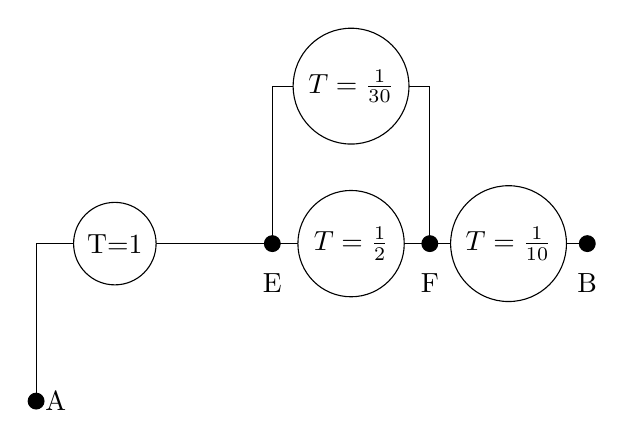
\begin{tikzpicture}
\filldraw (0,-2) circle[radius=1 mm];
\node at (0.25,-2) {A};
\draw (0,-2)--(0,0)--(1,0)node[circle, draw=black,radius=2cm, fill=white]{T=1}
--(3,0); 
\draw (3,0)--(4,0)node[circle, draw=black,radius=2cm, fill=white]{$T=\frac{1}{2}$}
--(5,0)--(6,0)node[circle, draw=black,radius=2cm, fill=white]{$T=\frac{1}{10}$}
--(7,0);
\draw (3,0)--(3,2)--(4,2)node[circle, draw=black,radius=2cm, fill=white]{$T=\frac{1}{30}$}--(5,2)--(5,0);
\filldraw (3,0) circle[radius=1 mm];
\node at (3,-.5) {E};
\filldraw (5,0) circle[radius=1 mm];
\node at (5,-.5) {F};
\filldraw (7,0) circle[radius=1 mm];
\node at (7,-.5) {B};
\end{tikzpicture}
\caption{A Trust Network. The T's represents edges of Trust.}
\label{F:3T2}
\end{center}
\end{figure}

Since trust levels are the inverse of distrust levels, their series and parallel combinations would be as follows:

\begin{align}
D_T&=D_1+D_2&\rightarrow&\frac{1}{T_T}=\frac{1}{T_1}+\frac{1}{T_2}&\text{Series}
\end{align}
and..
\begin{align}
\frac{1}{D_T}=\frac{1}{D_1}+\frac{1}{D_2}&&\rightarrow&T_T=T_1+T_2&&\text{Parallel}
\end{align}
Notice that these relationship are exactly reversed from the series and parallel combinations that you get from using levels of distrust.\par
In electric circuits, we define the conductance (G) of a component to be the inverse of its resistance. The relationship between conductance and resistance is the same as the relationship between trust and distrust. Therefore it should not surprise you that we combine series and parallel combinations of conductance in the following way.

\begin{align}
G_T=G_1+G_2&\leftarrow&\text{parallel}\\
\frac{1}{G_T}=\frac{1}{G_1}+\frac{1}{G_2}&\leftarrow&\text{Series}
\end{align}


%%%%%%%%%%%%%%%%%%%%%%%%%%%%%%%%%%%%%%%%%%%%%%%%%%%%%%%%%
\subsection{Series and Parallel Combinations of Sources}
Consider two voltage sources connected in series and then in parallel as shown in Figure~\ref{F:3SSP}. In this section, we will see how to simplify combinations of sources.

\begin{figure}[H]
\begin{center}
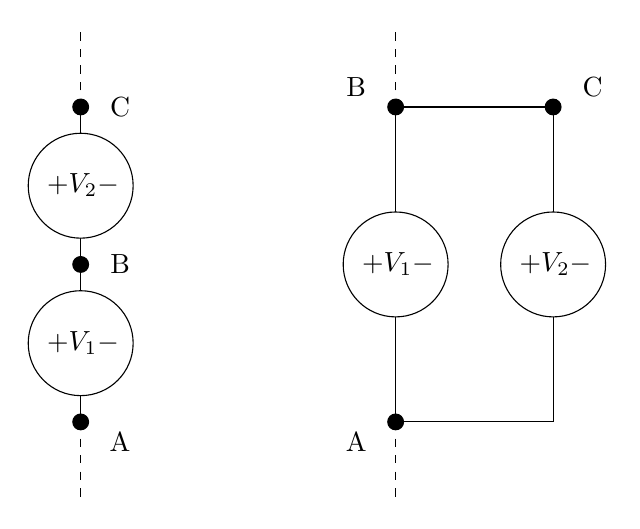
\begin{tikzpicture}
\filldraw (0,0) circle[radius=1 mm]; \draw node at (.5,-.25) {A};
\filldraw (0,2) circle[radius=1 mm]; \draw node at (.5,2) {B};
\filldraw (0,4) circle[radius=1 mm]; \draw node at (.5,4) {C};
\draw (0,0)--(0,1)node[circle, draw=black,radius=2cm, fill=white]{$\begin{matrix}+\\V_1\\-\end{matrix}$}
--(0,2); 
\draw (0,2)--(0,3)node[circle, draw=black,radius=2cm, fill=white]{$\begin{matrix}+\\V_2\\-\end{matrix}$}--(0,4);
\filldraw (4,0) circle[radius=1 mm]; \draw node at (3.5,-.25) {A};
\filldraw (4,4) circle[radius=1 mm]; \draw node at (3.5,4.25) {B};
\filldraw (6,4) circle[radius=1 mm]; \draw node at (6.5,4.25) {C};
\draw (4,0)--(4,2)node[circle, draw=black,radius=2cm, fill=white]{$\begin{matrix}+\\V_1\\-\end{matrix}$}
--(4,4); 
\draw (4,0)--(6,0)--(6,2)node[circle, draw=black,radius=2cm, fill=white]{$\begin{matrix}+\\V_2\\-\end{matrix}$}
--(6,4)--(4,4); 
\draw [dashed] (4,0)--(4,-1);
\draw [dashed] (4,4)--(4,5);
\draw [dashed] (0,0)--(0,-1);
\draw [dashed] (0,4)--(0,5);
\end{tikzpicture}
\caption{Series and Parallel Combinations of Voltage Sources}
\label{F:3SSP}
\end{center}
\end{figure}

Consider first the series combination. Apply KVL. Go around the following loop: start at A, go to B, up to C, then come back through the air \footnote{Some students feel uncomfortable thinking of the air as a legitimate path. Sure, it has a high resistance, but here's nothing wrong with it.} to A. Remember, $V_{BA}$ means $V_B-V_A$. Then:
\begin{align}
V_{BA}+V_{CB}+V_{AC}=0\\
V_{CA}=V_{BA}+V_{CB} =V_1+V_2 =V_{combined}
\end{align}
Voltage sources in series add.\par

On the other hand, the parallel combination presents the following problems:
\begin{itemize}
\item Apply KVL to the loop starting at A. Go up through V1 to B then down through V2 and then back to A. The sum of these voltages would only be zero if V1 matched V2. Otherwise, KVL is broken. Whoops.
\item Suppose you calculated the current from B to C. 
\begin{align}
I=\frac{\Delta V}{R}=\frac{V_1-V_2}{0} \rightarrow \infty
\end{align}
An infinite current is a problem. It would lead to infinite magnetic fields, require more than all the charge in the Universe, etc...
\end{itemize}
Ideal voltage sources of different amounts should not be combined in parallel. Real ones shouldn't either. Real world voltage sources have some internal resistance that would prevent infinite currents and prevent a breakdown of KVL, but they might still overheat or break or cause a fire.

\begin{clevel}
How would two current sources combine in parallel? How about two current sources in series?
\end{clevel}

%%%%%%%%%%%%%%%%%%%%%%%%%%%%%%%%%%%%%%%%%%%%%%%%%%%%%%%%
\section{Application: Two chain saws}
Suppose you and a friend want to cut up some brush. You both have 1.25 hp electric chain saws. You use a 14-gauge 100' extension cord and then send it to a power strip in your backyard. You then plug in both chain saws into the power strip. The chain saws are designed to operate with 120V, but will work so long as the voltage does not dip below 100V. What is the actual voltage at the chain saw if the outlet is at 115V?
\par
Let's make a model for this situation. We'll leave the third prong off the diagram; that wire is needed for safety but won't effect our calculations.

\begin{figure}[H]
\begin{center}
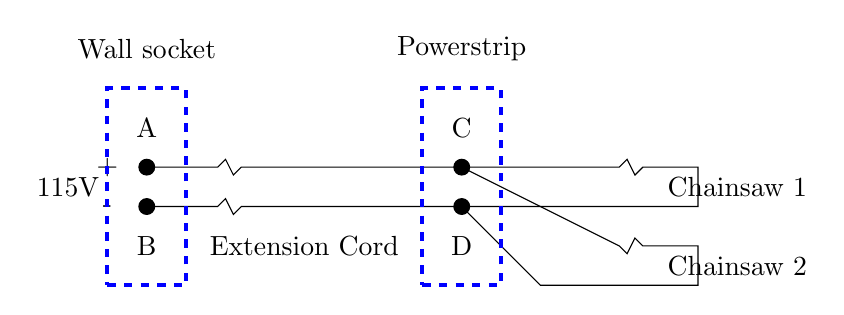
\begin{tikzpicture}
\draw (0,0)--(.9,0)--(1,.1)--(1.1,-.1)--(1.2,0)--(4,0);
\filldraw (4,0) circle[radius=1 mm];
\draw (0,.5)--(.9,.5)--(1,.6)--(1.1,.4)--(1.2,.5)--(4,.5);
\filldraw (4,.5) circle[radius=1 mm];
\draw node at (0,1) {A};
\draw node at (0,-.5) {B};
\draw node at (4,1) {C};
\draw node at (4,-.5) {D};
\draw node at (-.5,0) {-};
\draw node at (-.5,.5) {+};
\draw node at (-1,.25) {115V};
\draw node at (2,-.5) {Extension Cord};
\draw node at (7.5,.25) {Chainsaw 1};
\draw node at (7.5,-.75) {Chainsaw 2};
\filldraw (0,.5) circle[radius=1 mm];
\filldraw (0,0) circle[radius=1 mm];
\draw (4,.5)--(6,.5)--(6.1,.6)--(6.2,.4)--(6.3,.5)--(7,.5)--(7,0)--(4,0);
\draw (4,.5)--(6,-.5)--(6.1,-.6)--(6.2,-.4)--(6.3,-.5)--(7,-.5)--(7,-1)--(5,-1)--(4,0);
\draw [dashed, draw=blue,line width= 0.5mm] (3.5,-1) --(4.5,-1)--(4.5,1.5)--(3.5,1.5)-- (3.5,-1);
\draw node at (4,2) {Powerstrip};
\draw [dashed, draw=blue,line width= 0.5mm] (-.5,-1) --(.5,-1)--(.5,1.5)--(-.5,1.5)-- (-.5,-1);
\draw node at (0,2) {Wall socket};
\end{tikzpicture}
\caption{Electrical model of two chainsaws plugged into a power strip}
\end{center}
\end{figure}

Nodes A and B are at the outlet. Nodes C and D are at the power strip somewhere in the backyard.
\par
We need to determine the resistance values for the extension cord and chainsaws. Look up the cross-sectional area of a 14-gauge wire and the resistivity of copper.
\par
\begin{align*}
R_{cord} &= \rho \frac{L}{A}\\
R_{cord}&=(1.68E-8) \Omega m \frac{30.48 m}{(2.08E-6) m^2} = 0.246 \Omega
\end{align*}

\begin{blevel}
Based on the values used in the abeve equation, is the extension cord made of copper or aluminum. How can you tell? 
\end{blevel}

To approximate the resistance of the chainsaws \footnote{The electric chainsaw would not be best modeled as a simple resistor, but would likely have some inductance.}, we will use the power requirement, which is specified at ~120V to determine the current. Then use values of the current and voltage and Ohm's Law to determine the resistance.
\par

\begin{align}
P=IV \rightarrow 1.25*745 = I*120 \rightarrow I=7.8 Amps\\
V = IR \rightarrow 120 = 7.8*R \rightarrow R = 15.46 \Omega
\end{align}

Now, we'll use our tools to determine the voltage across the chainsaws.

\begin{enumerate}
\item Combine the two chainsaw resistances. Observe that they are in parallel. $R_{combined} = 7.73 \Omega$
\item The combined chainsaw resistance is then in series with the two extension cords resistances. Combining these gives one resistance of $R_T=8.22 \Omega$
\item Use Ohm's Law to determine the current entering the positive wire of the extension cord. I = 13.99 A.
\item Go back to the unsimplified circuit and use Ohm's Law to determine the voltage drop across the two legs of the extension cord. $V_{cordLeg} =3.44 V$
\item Use KVL to determine the voltage drop across one of the chainsaws. $+115V - 3.44 - V_{saw} - 3.44 = 0$. So, $V_{saw}=108.1 V$ 
\item Conclusion: The voltage does not dip below 100V, so the chainsaws should be OK.
\end{enumerate}

\begin{blevel}
Suppose a third chainsaw were plugged into the power strip. What would the voltage be across each operating chainsaw?
\end{blevel}

\begin{clevel}
What is the combined resistance of N identical resistors connected in parallel?
\end{clevel}

\begin{clevel}
Suppose N chainsaws were plugged into the power strip. Each chainsaw using P Watts of power, and the 14-gauge copper extension cord is now L meters long. Determine the voltage across each chainsaw in terms of P, L and N.
\end{clevel}

%%%%%%%%%%%%%%%%%%%%%%%%%%%%%%%%%%%%%%%%%%%%%%%%%%%%%%%%%%%%
\section{Voltage Division}
Now that we have established some basic tools, it might be worthwhile to look at a common situation in detail. You will encounter this situation often, so it is profitable to be quick at its analysis.
\par
The situation involves two resistors connected in series.
\par
\begin{figure}[H]
\begin{center}
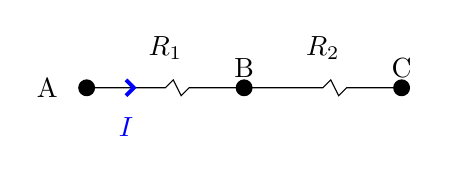
\begin{tikzpicture}
\node at (2,.5) {$R_1$};
\node at (4,.5) {$R_2$};
\filldraw (1,0) circle[radius=1 mm];
\node at (.5,0) {A};
\filldraw (3,0) circle[radius=1 mm];
\node at (3,.25) {B};
\filldraw (5,0) circle[radius=1 mm];
\node at (5,.25) {C};
\draw (1,0)--(2,0)--(2.1,.1)--(2.2,-.1)--(2.3,0)--(3,0);
\draw (3,0)--(4,0)--(4.1,.1)--(4.2,-.1)--(4.3,0)--(5,0);
\draw [draw=blue, line width=0.5mm] (1.5,.1)--(1.6,0)--(1.5,-.1);
\node [text=blue] at (1.5,-.5) {$I$};
\end{tikzpicture}
\caption{The basic voltage division situation}
\end{center}
\end{figure}

Imagine going around a loop where we start at A, go around through the air to C, then from C to B and then from B back to A. KVL says that the total voltage drop around this loop must be zero.
\par
\begin{align*}
V_{AC} + V_{CB}+V_{BA}&=0\\
V_{AC} &=-V_{CB}-V_{BA}\\
V_{AC} &= V_{AB}+V_{BC} \tag{Individual Voltages Sum to Total Voltage}\\
\end{align*}

Solve for $I_1$ then voltage across $R_1$, called $V_{AB}$:

\begin{align}
V_{AC} &= V_{AB}+V_{BC}\notag\\
V_{AC} &= IR_1+IR_2 \rightarrow I=\frac{V_{AC}}{R_1+R_2}\notag\\
V_{AB}&=IR_1\notag\\
V_{AB}&=\frac{V_{AC}}{R_1+R_2}R_1\notag\\
V_{AB}&=\frac{R_1}{R_1+R_2}V_{AC}
\end{align}

We conclude that a fraction ($\frac{R_1}{R_1+R_2}$) of the total voltage is dropped across $R_1$. That fraction is the same as the fraction of the total series resistance that is $R_1$.
\par


\begin{alevel}
Suppose $V_{AC}$ were 18 V and $R_1$ were 5 $\Omega$ and $R_2$ were 10 $\Omega$. How much voltage would be dropped across $R_1$? What about $R_2$?
\end{alevel}

\begin{blevel}
Suppose $V_{AC}$ were 18 V and $R_1$ were 5 $\Omega$ and $R_2$ were 10 $\Omega$.\\
What is $V_{AB}+V_{BC}$?\\
What is $V_{AB}+V_{BA}$?\\
What is $V_{AB}+V_{CB}$?
\end{blevel}

\begin{dlevel}
Prove that for N resistors in series, the voltage drop across $R_i$ is:
\par
\[ V_i=\frac{R_i}{(\sum\limits_{j=1}^{j=N} R_j)}V_{TOTAL} \]
\end{dlevel}

Consider a more complicated circuit like that shown in Figure~\ref{F:3VD}. Use voltage division to find the voltage across the 2 Ohm ($V_2$)resistor as follows:

\begin{enumerate}
\item Determine the fraction that $V_2$ is of $V_{BC}$. Answer: $V_2=\frac{2}{2+3}V_{BC}$
\item Determine the fraction that $V_{BC}$ is of $V_{AC}$. Answer: $V_{BC}=\frac{R_{BC}}{R_{BC}+5}V_{AC}$
\item Identify $R_{BC} = (2+3) \parallel 7$ $\Omega$
\item String it all together: 
\begin{align}
V_2=(\frac{2}{2+3})(\frac{(2+3) \parallel 7}{(2+3) \parallel 7+5})V_{AC}
\end{align}
\end{enumerate}

\par
\begin{figure}[H]
\begin{center}
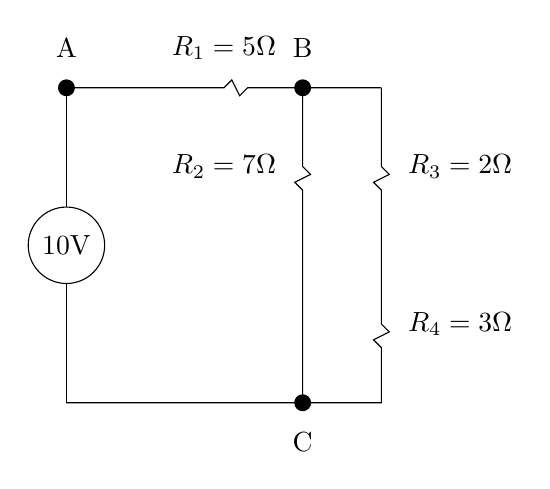
\begin{tikzpicture}
\node at (2,4.5) {$R_1=5\Omega$};
\node at (2,3) {$R_2=7\Omega$};
\node at (5,3) {$R_3=2\Omega$};
\node at (5,1) {$R_4=3\Omega$};
\filldraw (0,4) circle[radius=1 mm];
\node at (0,4.5) {A};
\filldraw (3,4) circle[radius=1 mm];
\node at (3,4.5) {B};
\filldraw (3,0) circle[radius=1 mm];
\node at (3,-.5) {C};
\draw (0,0)--(0,2) node[circle, draw=black, fill=white] {10V}--(0,4);
\draw (0,4)--(2,4)--(2.1,4.1)--(2.2,3.9)--(2.3,4)--(3,4)--(4,4);
\draw (4,4)--(4,3)--(4.1,2.9)--(3.9,2.8)--(4,2.7)--(4,2)
--(4,1)--(4.1,.9)--(3.9,.8)--(4,.7)--(4,0)--(0,0);
\draw (3,4)--(3,3)--(3.1,2.9)--(2.9,2.8)--(3,2.7)--(3,0);
\end{tikzpicture}
\caption{Circuit for practicing voltage division.}
\label{F:3VD}
\end{center}
\end{figure}

\begin{blevel}
Finish the calculation and get a value for the voltage across the 2 Ohm resistor. What is the current through it? 
\end{blevel}

\begin{clevel}
Use voltage division to determine the voltage across the 7 Ohm resistor in Figure~\ref{F:3VD}. 
\end{clevel}

\begin{clevel}
Use voltage division to determine the voltage across the 3 Ohm resistor in Figure~\ref{F:3VD}. 
\end{clevel}
%%%%%%%%%%%%%%%%%%%%%%%%%%%%%%%%%%%%%%%%%%%%%%%%%%%%%%%%%%%%%%%%%
